\documentclass[12pt]{article}

\usepackage{scicite,times,graphicx,float,hyperref}
\usepackage[skip=0pt]{caption}
\usepackage[utf8]{inputenc}
\usepackage{enumitem}
\usepackage{booktabs}

\topmargin -1.0cm
\oddsidemargin 0.0cm
\textwidth 16cm 
\textheight 23cm
\footskip 1.0cm

\newenvironment{sciabstract}{%
\begin{quote} \bf}
{\end{quote}}

\newcounter{lastnote}
\newenvironment{scilastnote}{%
  \setcounter{lastnote}{\value{enumiv}}%
  \addtocounter{lastnote}{+1}%
  \begin{list}%
  {\arabic{lastnote}.}
  {\setlength{\leftmargin}{.22in}}
  {\setlength{\labelsep}{.5em}}
}
{\end{list}}

\title{A Farm Simulation\\using Swing and Concurrency} 

\author
{Filipe Pires [85122], João Alegria [85048]\\
\\
Software Architecture\\
\normalsize{Department of Electronics, Telecommunications and Informatics}\\
\normalsize{University of Aveiro}\\
} 

\date{\today{}}

%%%%%%%%%%%%%%%%% END OF PREAMBLE %%%%%%%%%%%%%%%%

\begin{document} 

\baselineskip18pt

\maketitle 

\section{Introduction} %%%%%%%%%%%%%%%%%%%%%%%%%%%%%%%%%%%%%%%%%%%%%%%%%%%%%%%%%%%%%%%%%%%%%%%%%%%%%%%%%%%%%%%%%%%%%%%%%%%%%%%%%%%%%%%%%%%%%%%%%%%%%%%%%%%%%%%%%

This report aims to describe the work developed for the first assignment of the course of 'Software Architecture', explaining the overall architecture and 
describing its components and respective communication channels and elaborating on the adopted solutions for concurrency.
We also mention how the work was distributed amongst the authors.

The Java application has the purpose of conducting harvest simulations on an agricultural farm.
Along with the technical aspects of the implementation, we also elaborate on the adopted solutions for concurrency.
Efforts on making the UI highly usable and the code readable and well documented are also stated here.
All code developed is publicly accessible in our GitHub repository: 

\url{https://github.com/FilipePires98/AS/}.
\newpage

\section{The Agricultural Farm} \label{farm} %%%%%%%%%%%%%%%%%%%%%%%%%%%%%%%%%%%%%%%%%%%%%%%%%%%%%%%%%%%%%%%%%%%%%%%%%%%%%%%%%%%%%%%%%%%%%%%%%%%%%%%%%%%%%%%%%%%

.....

% \vspace{0.2in}
% \begin{minipage}{0.45\textwidth}
%   \begin{verbatim}
%     def stringA():
%       for i in range(5):
%         print("01", end="")
%   \end{verbatim}
% \end{minipage}
% \begin{minipage}{0.45\textwidth}
%   \begin{verbatim}
%     def stringB():
%       for letter in "0010100110":
%         print(letter, end="")
%   \end{verbatim}
% \end{minipage}
% \vspace{0.2in}

% \begin{equation} \label{eq:1}
%   NID(x,y) = \frac{max\{K(x|y),K(y|x)\}}{max\{K(x),K(y)\}}
% \end{equation}

\subsection{Control Center} %%%%%%%%%%%%%%%%%%%%%%%%%%%%%%%%%%%%%%%%%%%%%%%%%%%%%%%%%%%%%%

........

\subsection{Farm Infrastructure} %%%%%%%%%%%%%%%%%%%%%%%%%%%%%%%%%%%%%%%%%%%%%%%%%%%%%%%%%

........

\newpage
\section{System Architecture} %%%%%%%%%%%%%%%%%%%%%%%%%%%%%%%%%%%%%%%%%%%%%%%%%%%%%%%%%%%%%%%%%%%%%%%%%%%%%%%%%%%%%%%%%%%%%%%%%%%%%%%%%%%%%%%%%%%%%%%%%%%%%%%%%%

.....

% \begin{figure}[H]
%   \centering
%   \begin{minipage}{\textwidth}
%     \centering
%     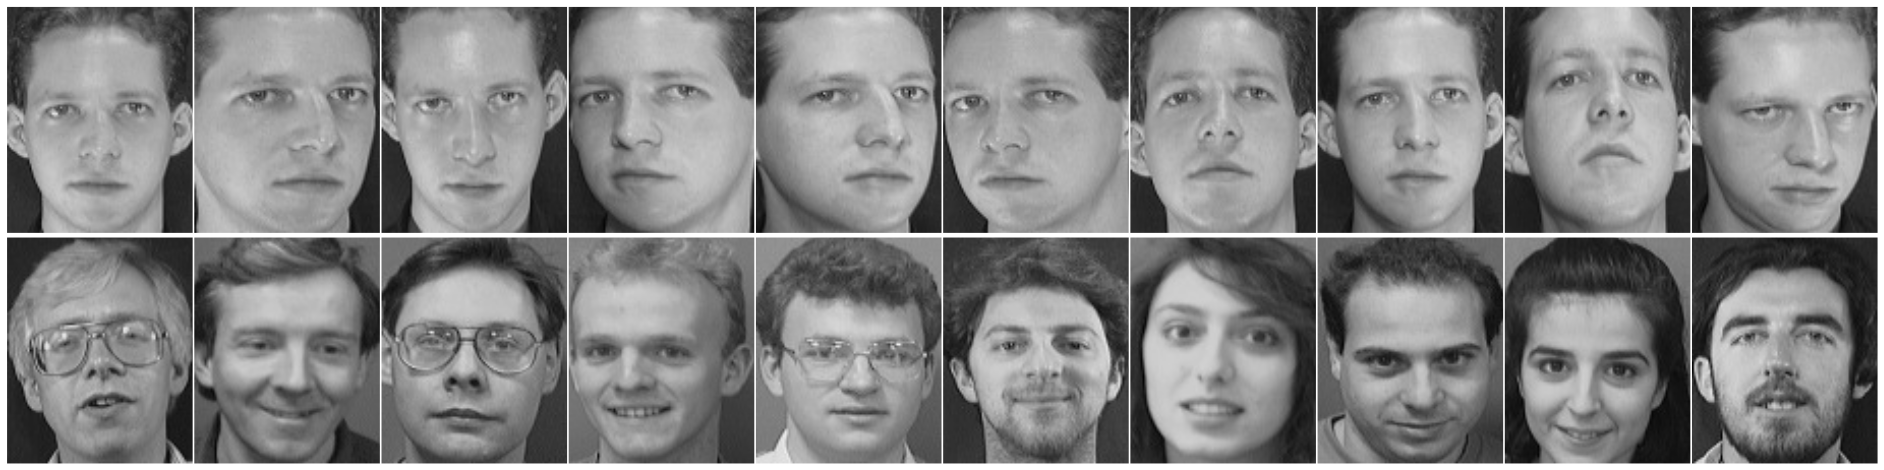
\includegraphics[width=\linewidth]{faces_example.png}
%   \end{minipage}%
%   \caption{Image taken from the assignment description \cite{trab3}. Examples from the ORL face dataset. In the first row, ten face images corresponding to the same subject (s01). In the second row, the first face image of subjects s02 to s11.}
%   \label{fig:1}
% \end{figure}

% \vspace{-10pt}
% \begin{itemize}[noitemsep]
%   \item Append - this operation unites the two images one above the other (duplicating the height of the resulting image).
%   \item Interlace - interpolated horizontal stripes of both images are stacked together (in this operation half of the data of each image is not used).
%   \item Average - for each pixel position, the average of the gray value of both images at that position is calculated and added to the new image in the same position.
% \end{itemize}
% \vspace{-10pt}

% \begin{table}[h!]
%   \centering
%   \begin{tabular}{@{}c|cccccc@{}}
%                      & \textbf{\texttt{zip}} & \textbf{\texttt{gzip}} & \textbf{\texttt{lzma}} & \textbf{\texttt{bzip2}} & \textbf{\texttt{zpaq}} & \textbf{\texttt{ppmd}}\\ \midrule
%   \textbf{Append}    & 0.707     & \textbf{0.725}   & 0.271           & 0.507     & 0.060           & 0.657 \\
%   \textbf{Interlace} & 0.100     & 0.560            & \textbf{0.682}  & 0.578     & 0.021           & 0.025 \\ 
%   \textbf{Average}   & 0.021     & 0.021            & 0.014           & 0.042     & \textbf{0.089}  & 0.025 \\ 
%   \end{tabular}
%   \vspace{5pt}
%   \caption{Accuracy for each compressor using different concatenation operations.}
%   \label{tab:1}
%   \end{table}

\subsection{Components} %%%%%%%%%%%%%%%%%%%%%%%%%%%%%%%%%%%%%%%%%%%%%%%%%%%%%%%%%%%%%%

........

\subsection{User Interface} %%%%%%%%%%%%%%%%%%%%%%%%%%%%%%%%%%%%%%%%%%%%%%%%%%%%%%%%%

........

\newpage
\section{Concurrency Strategy} %%%%%%%%%%%%%%%%%%%%%%%%%%%%%%%%%%%%%%%%%%%%%%%%%%%%%%%%%%%%%%%%%%%%%%%%%%%%%%%%%%%%%%%%%%%%%%%%%%%%%%%%%%%%%%%%%%%%%%%%%%%%%%%%%

.....

\subsection{Communications} %%%%%%%%%%%%%%%%%%%%%%%%%%%%%%%%%%%%%%%%%%%%%%%%%%%%%%%%%

........

\subsection{Farmers} %%%%%%%%%%%%%%%%%%%%%%%%%%%%%%%%%%%%%%%%%%%%%%%%%%%%%%%%%%%%%%

........

% \begin{verbatim}
%   for each compressor, do:
%     for each subject, do:
%       minNCD = 1
%       for each testImg, do:
%         for each goldStdImg, do:
%           tmp = concat(testImg,goldStdImg)
%           cTmp = compress(tmp)
%           cT = compress(testImg)
%           cGS = compress(goldStdImg)
%           maxS = getMaxSize(cTmp,cT,cGS)
%           minS = getMinSize(cTmp,cT,cGS)
%           NCD = (size(cTmp) - minS) / maxS
%           if NCD < minNCD:
%             minNCD = NCD
% \end{verbatim}

\newpage
\section{Documentation} %%%%%%%%%%%%%%%%%%%%%%%%%%%%%%%%%%%%%%%%%%%%%%%%%%%%%%%%%%%%%%%%%%%%%%%%%%%%%%%%%%%%%%%%%%%%%%%%%%%%%%%%%%%%%%%%%%%%%%%%%%%%%%%%%%%%%%%%

.....

\newpage
\section{Discussion} %%%%%%%%%%%%%%%%%%%%%%%%%%%%%%%%%%%%%%%%%%%%%%%%%%%%%%%%%%%%%%%%%%%%%%%%%%%%%%%%%%%%%%%%%%%%%%%%%%%%%%%%%%%%%%%%%%%%%%%%%%%%%%%%%%%%%%%%%%%

.....

Regarding the work distribution amongst developers, a close-contact strategy was defined where each worked on a piece of software according to a predefined plan. 
The project structure and architecture was decided in conjunction, as well as the key concurrency solutions chosen.

Nevertheless, some relatively independent task distribution was defined: João implemented the Granary and Path monitors, while Filipe did the Storehouse and 
Standing monitors; João established socket communications and respective message processors, while Filipe designed the user interface and respective interaction
with the remaining components.
Bug and error solving was made along the development phase by both developers any time it was required.

Once the final version of the application was completed, this report and the code documentation became our primary concern, with both contributing equally.


\newpage
\section{Conclusions} %%%%%%%%%%%%%%%%%%%%%%%%%%%%%%%%%%%%%%%%%%%%%%%%%%%%%%%%%%%%%%%%%%%%%%%%%%%%%%%%%%%%%%%%%%%%%%%%%%%%%%%%%%%%%%%%%%%%%%%%%%%%%%%%%%%%%%%%%%

After completing the assignment, we drew a few conclusions regarding the topics here explored and our endeavor to deliver work of quality.

.....

\begin{thebibliography}{9} %%%%%%%%%%%%%%%%%%%%%%%%%%%%%%%%%%%%%%%%%%%%%%%%%%%%%%%%%%%%%%%%%%%%%%%%%%%%%%%%%%%%%%%%%%%%%%%%%%%%%%%%%%%%%%%%%%%%%%%%%%%%%%%%%%%%%
  \bibliographystyle{Science}

  \bibitem{trab3}
    Óscar Pereira,
    \textit{SA: Practical Assignment no.1},
    University of Aveiro,
    2019/20.
  
  % \bibitem{imgmagick}
  %   ImageMagick Studio LLC,
  %   \textit{ImageMagick},
  %   \url{https://imagemagick.org/index.php},
  %   accessed in December 2019.

  % \bibitem{lzmaExplanation}
  %   Borbely, R.,
  %   On normalized compression distance and large malware: Towards a useful definition of normalized compression distance for the classification of large files,
  %   Journal of Computer Virology and Hacking Techniques,
  %   2015,
  %   10.1007/s11416-015-0260-0
  %   \url{https://www.researchgate.net/publication/290319316_On_normalized_compression_distance_and_large_malware_Towards_a_useful_definition_of_normalized_compression_distance_for_the_classification_of_large_files},
  %   accessed in December 2019.
  
\end{thebibliography}

\clearpage

\end{document}




















